\section{Algorithms implemented}
\label{alg}
While various EA are suitable for optimizing ES, the final selection for this study consists of the Genetic Algorithm (GA), the Backtracking Search Algorithm (BSA), Population-based Incremental Learning (PBIL) and Particle Swarm Optimization (PSO). As a benchmark of performance Hil-Climbing and Stochastic Hill-Climbing are implemented.

\subsection{Genetic Algorithm}
%\ref{GA}
As the Genetic Algorithm (GA) has already been explained in its canonical form in Section \ref{introEA} as a prototype of EAs, it will not be dealt with in much detail. For the ES case, a GA with elitism, one-point crossover and roulette-wheel selection is implemented.


\subsection{Backtracking Search Optimization Algorithm}
%ref{BSA}
The Backtracking Search Optimization Algorithm (BSA) is comparatively new algorithm that was introduced in 2013 to solve numerical problems \citep{civicioglu2013backtracking}. Out of all the algorithms taken into account, it can be considered the``sleekest" with only one control parameter. Additionally to the GA phases, a second Selection stage is implemented at the very beginning where an old population is maintained such that the BSA population preserves a memory. 
After initialization follows the new selection stage where the historical population is randomly updated according to $\textit{if } a < b  \:|\: a,b \sim U(0,1 )$. It is then permuted and Mutation and Crossover follow. The population is mutated based on Equation (\ref{eqbsa1}):
\begin{equation} \label{eqbsa1}
\textit{Mutant} = \textit{Population} + F \cdot (\textit{historical Population} - \textit{Population})
\end{equation}
where $F = 3 \cdot \varepsilon$, $\varepsilon \sim N(0,1)$.
The original BSA is developed for numerical, real-valued problems but it can easily be adapted to binary encoding.

\subsection{Population-Based Incremental Learning}
%ref{PBIL}
The Population-Based Incremental Learning Algorithm (PBIL) by \cite{baluja1994population} can be considered an abstraction of the GA as it drops the population. Instead, it uses a probability vector from which population samples are drawn. This vector denotes the probability of a certain value appearing at a certain position of the solution vector. In a binary setting of the PBIL, the probability vector of a population denotes the probability of a 1 appearing at position $i$ of the candidate solution $x$. Instead of recombination to obtain solutions with high fitness, the probability vector from which the population is drawn is gradually shifted towards solutions with high fitness \cite[p. 11]{baluja1994population}. The vector is initialized with 0.5 and is updated by the following rule:
\begin{equation}
p_i = p_i \cdot (1 - \gamma) + (\gamma \cdot x_i),
\end{equation}
where $p_i$ is the probability of generating a 1 bit at position $i$, $x_i$ is the solution vector at position $i$ towards which the probability vector at $i$ is moved and $\gamma$ is the learning rate. The learning rate affects how quickly the probability vector moves towards a feasible solution, i.e. how informative the previous search is. As such, it controls the trade-off between exploration and exploitation and premature convergence. It is usually suggested to set the learning rate to values around 0.1, as higher values lead to an early search focus whereas lower values enable greater search exploration, which is preferable when there is no certainty on the prevalence of local optima. \cite[p. 16--17]{baluja1994population}.
It should be noted that the PBIL and the probability vector so far are as described in \cite{baluja1994population}, meaning that only binary encoding is considered. The PBIL, however, can be adapted to real-valued encoding, thus making the implication of a probability vector more complicated. 

As a solution, \cite{servet1997telephone} suggest an interval-based probability vector. It is assumed that the solution is continuous and bounded, such that for each position $i$, an bounded interval $[low_i, up_i]$ can be defined. The value at position $i$ of the probability vector then denotes the probability that $x_i$ is greater than a threshold. The initial threshold is defined as $\frac{low_i + up_i}{2}$ and is updated throughout the iterations. If $p_i \geq 0.9$, i.e. the probability that $x_i$ is greater than the threshold is $\geq 0.9$, the threshold is updated to $\frac{\frac{low_i + up_i}{2} + up_i}{2}$, i.e. $low_i$ is updated to the previous threshold and $p_i$ is reinitialized at 0.5. Both $p_i$ and the $up_i$ are updated equivalently whenever $p_i \leq 0.1$. In the case of ES in this pape, the interval is slightly redefined from $\frac{low_i + up_i}{2}$ to $\frac{low_i + up_i}{\sum{i}}$ such that the initial probability assumes equal weights.



\subsection{Particle Swarm Optimization}
%ref{PSO}
The Particle Swarm Optimization Algorithm (PSO) draws on swarm intelligence to find the optimum. The candidate solutions, called particles, move through the search space by random mutations, called velocities. The velocity of each particle consists of three components: an inertia weight, i.e. the "unwillingness" of a particle to leave its current position which also prevents it from moving too erratically, a cognitive component, i.e. the particle's ability to remember a previous good solution, and a social component, i.e. the particle's ability to move towards optimal solutions found by its neighbors in the swarm. 
The PSO was introduced in 1995 by Kennedy and Eberhart and simulates the social behavior of bird flocking or fish swarming. 
The particles evolve by the following equations:
\begin{align}
v_{i,t+1} &= \gamma v_{i,t} + \varphi_1 \delta(0,1)(P_i - x_{i,t}) + \varphi_2 \delta(P_g - x_{i,t})\\
x_{i,t+1} &= x_{i,t} + v_{i,t+1}
\end{align}
where $\delta \sim U(0,1)$, $x_{i,t}$ is the value at position $i$ and time step $t$ of the candidate solution $x$, $P_i$ refers to the previously best personal solution and $P_g$ denotes the best solution in the neighborhood. \\
The inertia weight $\gamma$ controls how fast each particle moves and was not in the proposition for the original PSO \citep{kennedy1995}. It was added three years later as it adds significantly to the algorithm's ability to search and exploit the search space \cite[p. 70]{shi1998modified}. For $\gamma > 1.2$ the swarm keeps on exploiting new search areas, for $\gamma < 0.8$ it exploits local areas more and finds the balance between the two for values $0.8 < \gamma < 1.2$ However, experimental studies have shown that non-fixed $\gamma$ values also perform extremely well and that the so called random inertia weight $\gamma = 0.5 + \delta/2$ performs well on a number of different problems \cite[p. 643]{bansal2011inertia}.
$\varphi_1$ and $\varphi_2$, the acceleration coefficients control the influence of information on the movement of the particles. Usually, one sets $\varphi_1 = \varphi_2$ to values around 2 \cite[p. 1946]{kennedy1995}. \\
Additionally, the information neighborhood of each particle, also called topology, is not a trivial setup as it determines how much information is available to each particle. The two most common ones are the \textit{lbest} and \textit{gbest} topologies but there are many other variants. In the \textit{lbest}, each particle $i$ is informed on its own position and its two adjacent neighbors, resulting in a ring lattice (see Figure \ref{Fig:topo}). In a \textit{gbest} setting, which is also the setting in the initial algorithm, the particles are informed by the global neighborhood. The information flow in this social network influences the convergence behavior strongly: In a study by \cite{kennedymendes}, different topologies were evaluated and \textit{gbest} performed worst in both accuracy and speed, while \textit{lbest} performed slightly better when removing particle $i$ (the self) from the information \cite[p. 1674]{kennedymendes}. For this paper, both the \textit{gbest} and \textit{lbest} without self are tested; more complex topologies von Neumann neighborhood were not considered due to the popularity of the former and the complexity of the latter.

\begin{figure}[ht]
	\begin{center}
		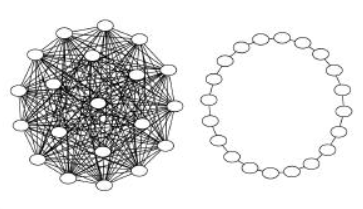
\includegraphics[scale=0.9]{topology}
		\caption{A visualization of the \textit{gbest} and \textit{lbest} topologies \cite[p. 1671]{kennedymendes}.}
		\label{Fig:topo}
	\end{center}
\end{figure}



\subsection{(Stochastic) Hill-climbing}
Simple Hill-climbing is an iterative search algorithm that does not belong to the class of evolutionary algorithms. It is, however, a powerful and fast algorithm that XXX.
HC systematically modifies an initial candidate solution in directions that yield higher fitness values. If the first modification did not improve the current fitness value, the solution moves into another direction. Ideally, in a convex space with only one optimum, HC returns the hill-top, the best solution after a fixed number of iterations \cite[p. 252]{skiena2008algorithm}. As solutions with lower fitness values are not further investigated, HC is prone to get stuck in local optima as it cannot return to previous points and must go upwards \cite[p. 113]{russell1995modern}. 
One resolution to mitigate this problem is Stochastic Hill-climbing where a random neighbor around the current solution is selected and evaluated. If it yields higher fitness, it replaces the current solution. instead of systematic mutation, randomly mutated candidate are evaluated and accepted if they yield a higher fitness. With this probabilistic element, the HC is forced to consider solutions further away from the current solution.

Both the simple HC and the SHC are simple to implement and perform very well on a number of optimization problems \citep{Jacobson2004}. They are often used as benchmark comparisons because one can justify (or fail to justify) the use of more complex algorithms like EAs when simpler and faster methods like HC perform competitively (\cite{mitchell1993will}, \cite{wattenberg1996stochastic}, \cite{PRUGELBENNETT2004135}).





\section{Experimental Design}
\label{design}
All algorithms were hand-coded in R and tested on the publicly available data from the DATA MINING CUP 2016 on fashion retail returns was used \citep{dmcdata}. As in the contest submissions of Humboldt University of Berlin, a model library of 26 Random Forests and 26 XGBoost, 54 models in total, was used. 
The high server usage at the Research Data Center at Humboldt University where all computations for this paper were handled limited both the variety of different parameter settings, the number of iterations and the data sets on which the algorithms were run. 
To deal with these restrictions, the DMC data set was reduced to 30\% of its original size. This sub-set was then split into a training and a validation set with a 70/30 ratio, so that each algorithm optimized on 372,000 predictions. The evaluation of the optimization function, which is usually called several times in each iteration of the evolutionary algorithms is quite computationally expensive, so that even with the reduced data set, the number of iterations was limited to 500.


Each configuration of the five evolutionary algorithms was optimized in four seperate experiments: 1. binary-encoded, 2. real-valued, 3. binary-encoded + Bagging and 4. real-valued + Bagging. Bagging used of ten bags each.

All experiments followed the same structure: the solution populations were optimized over 500 generations (or iterations) where their performance was evaluated on a validation set. As a performance measure, the Brier Score was used, which can be intuitively understood a version of the Mean Squared Error for binary outcomes. It is defined as:
\begin{equation}
BS = \frac{1}{N} \sum_{i = 1}^{N} (p_i - o_i)^2
\end{equation}
where $N$ denotes the sample size, $p_i$ is the predicted probability and $o_i$ is the actual binary outcome (i.e. 1 or 0). The Brier Score lies in the [0,1] interval where a low value indicates a good forecast and the higher the Brier Score, the poorer the forecast performance. In the Bagging experiments, each algorithm is optimized on ten different subsets of the full classifier set and the results are then averaged.
Additionally, the ensemble weights yielded by the algorithms were tested on the classification set of the DMC. The results for this data were recently published and are available on the DMC website.
\begin{table}[ht]
	\centering
	\begin{tabular}{llcccc}
		\hline
		
		Algorithms& Abbr. & Psize & \multicolumn{3}{c}{Parameters} \\ 
		\hline
		& & & Mixrate& & \\
		\multirow{2}{*}{BSA} & BSA1 & 30 & 1 && \\ 
		& BSA2 & 100 & 1&& \\ \hline
		& & & Crossover & Elitism & pMutation \\
		\multirow{4}{*}{GA}  & GA1 & 30 & 0.50 & 0.03 & 0.05 \\ 
		& GA2 & 100 & 0.50 & 0.03 & 0.05 \\ 
		& GA3 & 30 & 0.80& 0.03 & 0.05 \\ 
		& GA4 & 100 & 0.80& 0.03 & 0.05 \\ \hline 
		 &&& Learning Rate & Shift & Prob \\
		\multirow{4}{*}{PBIL} & PBIL1 & 30 & 0.05& 0.05 & 0.02 \\ 
		& PBIL2 & 100 & 0.05 & 0.05 & 0.02\\ 
		& PBIL3 & 30 & 0.10& 0.05 & 0.02 \\ 
		& PBIL4 & 100 & 0.10 & 0.05 & 0.02 \\ \hline 
		 &&& Phi & Inertia & Initial Speed \\
		\multirow{4}{*}{PSO-G} & PSOG1 & 30 & 1.80 & 0.5 + $\delta$/2 & 0.01 \\ 
		&PSOG2 & 100 & 1.80& 0.5 + $\delta$/2 & 0.01 \\ 
		&PSOG3 & 30 & 2.10 & 0.5 + $\delta$/2 & 0.01\\ 
		&PSOG4 & 100 & 2.10& 0.5 + $\delta$/2 & 0.01 \\ \hline
		 &&& Phi & Inertia & Initial Speed \\
		\multirow{4}{*}{PSO-L} & PSOL1 & 30 & 1.80& 0.5 + $\delta$/2 & 0.01 \\ 
		& PSOL2 & 100 & 1.80& 0.5 + $\delta$/2 & 0.01 \\ 
		& PSOL3 & 30 & 2.10 & 0.5 + $\delta$/2 & 0.01\\ 
		& PSOL4 & 100 & 2.10 & 0.5 + $\delta$/2 & 0.01 \\ 
		\hline
	\end{tabular}
\caption{The parameter configurations for each variant of the five evolutionary algorithms run; $\delta \sim U(0,1)$}
\label{tbl:params}
\end{table}


